Աշխատանքի երկրորդ գլուխը նվիրված է գրաֆների դեկարտյան արտադրյալների միջակայքային ներկումներին: 
$G$ և $H$ գրաֆների $G\square H$ դեկարտյան արտադրյալը սահմանվում է հետևյալ կերպ.
\begin{align*}
V(G \square H) &= V(G) \times V(H),\\
E(G \square H) &= \left\{(u_1,v_1)(u_2,v_2) : (u_1=u_2 \text{ և } v_1v_2 \in E(H)) \text{ կամ } (v_1=v_2 \text{ և } u_1u_2 \in E(G) \right\}:
\end{align*} 

Հայտնի է\footnote{K. Giaro, M. Kubale, Compact scheduling of zero-one time operations in multi-stage systems, Discrete Appl. Math. 145, 2004, pp. 95-103.}, որ եթե $G,H\in \mathfrak{N}$, ապա $G\square H\in \mathfrak{N}$, ընդ որում,
$w(G\square H)\leq w(G)+w(H)$ և $W(G\square H)\geq W(G)+W(H)$:

\begin{hide}
\begin{theorem}\cite{GiaroKubale2004,Kubale2004}
\label{t2_cartesian} Եթե $G,H\in \mathfrak{N}$, ապա $G\square H\in \mathfrak{N}$. Ընդ որում,
$w(G\square H)\leq w(G)+w(H)$ և $W(G\square H)\geq W(G)+W(H)$:
\end{theorem}

\begin{theorem}\cite{Petrosyan2011}
\label{t2_kotzig} Եթե $G$ և $H$ գրաֆները համասեռ են և տեղի ունի հետևյալ պայմաններից գոնե մեկը.
\begin{enumerate}
\item $G$-ն և $H$-ը ունեն կատարյալ զուգակցում,
\item $G\in \mathfrak{N}$,
\item $H\in \mathfrak{N}$,
\end{enumerate}
ապա $G \square H \in \mathfrak{N}$:
\end{theorem}
\end{hide}
2.1 պարագրաֆում ուսումնասիրվել է միջակայքային ներկում չունեցող գրաֆների մասնակցությամբ դեկարտյան արտադրյալների ներկելիության հարցը: Ստացված արդյունքները ամփոփված են Աղյուսակ \ref{table2-cartesian}-ում:

\begin{hide}
\begin{lemma}
\label{l2-cartesian-eulerian}
Եթե $G$-ն էյլերյան գրաֆ է, ունի զույգ թվով կողեր և կենտ թվով գագաթներ, իսկ $H$-ը կենտ թվով կողեր ունեցող էյլերյան գրաֆ է, ապա $G \square H$ արտադրյալը ևս էյլերյան է և ունի կենտ թվով կողեր:
\end{lemma}
\begin{proof}[Ապացույց]
$G\square H$ գրաֆը ակնհայտորեն էյլերյան է: Իսկ արտադրյալի կողերի քանակը՝ $|E(G \square H)| = |E(H)||V(G)| + |E(G)||V(H)|$, կենտ է, քանի որ $|E(G)|$-ն զույգ է, իսկ $|E(H)|$-ը և $|V(G)|$-ն՝ կենտ:
\end{proof}
\end{hide}
\begin{table}[h]
    \centering
    \begin{tabular}{c|c|c}
         & $G \square H \in \mathfrak{N}$ & $G \square H \notin \mathfrak{N}$ \\
         \hline
        $G \in \mathfrak{N}$, $H \in \mathfrak{N}$ & $G=H=K_2$ & հնարավոր չէ \\
        $G \in \mathfrak{N}$, $H \notin \mathfrak{N}$ & $G=K_2$, $H=K_3$ & $G=$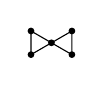
\begin{tikzpicture}[baseline=-0.5ex]
        \draw[fill=black] (0:0) circle(1pt);
        \draw[fill=black] (30:0.3cm) circle(1pt);
        \draw[fill=black] (-30:0.3cm) circle(1pt);
        \draw[fill=black] (150:0.3cm) circle(1pt);
        \draw[fill=black] (-150:0.3cm) circle(1pt);
        \draw (30:0.3cm) -- (0:0) -- (150:0.3cm) -- (-150:0.3cm) -- (0:0) -- (-30:0.3cm) -- cycle;
        \end{tikzpicture}, $H=K_3$ \\ 
        $G \notin \mathfrak{N}$, $H \notin \mathfrak{N}$ & $G=H=P_{10}$ & $G=H=K_3$ \\ 
        
    \end{tabular}
    \caption{Գրաֆների դեկարտյան արտադրյալների միջակայքային ներկելիության հարաբերությունը առանձին բաղադրիչների միջակայքային ներկելիության հետ՝ օրինակներով:}
    \label{table2-cartesian}
\end{table}

